%------------------------------------------------------------
%生涯学習基盤経営 TeXテンプレート Ver. 2.1
%arranged by Fukuji IMAI
%改訂内容:
%・英語タイトルの誤記,氏名および所属見本の改訂を行った。
%------------------------------------------------------------
%生涯学習基盤経営 TeXテンプレート Ver. 2
%arranged by Fukuji IMAI
%改訂内容:
%・スタイルファイルVersion2を参照するようにした。
%・(スタイルファイルVersion2への対応)副題に対応するためにjtitleの引数を2つ取るようにした。
%・(スタイルファイルVersion2への対応)英語要約の行間広げ,字下げ対応のため,eabstract環境を新設。
%------------------------------------------------------------
\documentclass[b5paper,10pt,twocolumn,tombow]{jarticle}
\usepackage[size=a4paper,priority=high]{bxpapersize}
\usepackage{llls}
\usepackage[bold]{otf}
\usepackage{graphicx}
\urlstyle{rm}
\begin{document}
\twocolumn[
\voltitle{41}{2016}

\begin{center}
\jtitle{『生涯学習基盤経営』における論文等の執筆マニュアル}{---\LaTeX{}
 バージョン---}
\end{center}

\begin{authors}
\name{1}{本郷弥生}
\name{2}{東大太郎}
\end{authors}
\begin{affiliation}
 \aff{1}{東京大学大学院教育学研究科}
 \aff{2}{生涯学習基盤経営学会}
\end{affiliation}

\begin{center}
\begin{abstract}
この文章は『生涯学習基盤経営』の論文等(論文,研究ノート,資料)のレイアウ
 トを説明した文章です。この文章自体が執筆要領を兼ねておりますので,この
 ファイルをそのまま使用して論文を作成することを推奨します。
\end{abstract}
 \begin{keyword}
キーワード: 生涯学習基盤経営,執筆要領,レイアウト
\end{keyword}
\end{center}



\initialize
]
\tableofcontents{}
\bigskip{}
\section{はじめに}
この文章は『生涯学習基盤経営』の論文等(論文,研究ノート,資料)のレイアウ
トを説明した文章です。この文章自体が執筆要領を兼ねております。このファイ
ルをそのまま使用して論文を作成することを推奨します。本稿をよくお読みいた
だき,原稿を作成して下さい。


なお,このファイルでは\LaTeX{}のレイアウトが記載されています。
Microsoft Word(以下,Word)の
レイアウト規定を確認されたい場合には,Wordのテンプレートファイルをご参照
下さい。なお,本要領は情報メディア学会の執筆要項ファイルを参照しました
\footnote{情報メディア学会. 『情報メディア研究』への各種原稿の投稿につい
て. 入手先URL:\\ http://www.jsims.jp/toko.html, (2008--10--27参照)}。

\LaTeX{}のテンプレートファイルを使用する場合にはスタイルファイルが必要です。
テンプレートファイルのアーカイブにスタイルファイルが同封してあります。テ
ンプレートファイルと同じディレクトリに設置するか,\LaTeX{}のスタイルファイ
ル格納場所(環境によって異なります)に設置して利用してください。現在のス
タイルファイル名は``Lifelong10.sty''です。

\LaTeX{}の原稿執筆には環境,並びにコマンドを使用します。本テンプレートファ
イルにおいて,環境とは$\backslash$begin\{\}で始まり,$\backslash$end\{\}
で閉じる命令のことを指し,コマンドとは$\backslash$textit\{\}のように,引
数を伴う命令のことを指します。またコマンドによっては引数を複数取ることが
あります。例えば紀要の号数と出版年を記入する$\backslash$voltitleコマン
ドは
\begin{verbatim}
\voltitle{35}{2010}
\end{verbatim}
と2つの引数を取ります。本マニュアルでは,この2つの引数をコマンド
の左側からそれぞれ,第1引数,第2引数と呼ぶこととします。

\section{原稿について}
A4版を使用し,原則として投稿段階から\LaTeX{}あるいはMicrosoft社のWordによっ
て,原稿を作成してください。作成の際には,必ずテンプレートファイルに基づ
き,印刷原稿にトンボが適切に出力されるように,作成して下さい(紀要
はB5サイズで印刷されます)。

\section{全体的なレイアウトについて}
\subsection{段組および字数・行数}

本文に先行するヘッダーの部分(論文等タイ
トル,著者氏名,要約)および,英文要約については一段組で,本文については
二段組1行22字で,縦は44行程度で設定してください。\LaTeX{}の場合,本テンプレー
トの使用により,同等の出力が得られます。


\subsection{文字サイズと字体}
\LaTeX{}の文字サイズについては,スタイルファイルであるLifelong10.sty
によって定義されていますので,著者側で文字サイ
ズの変更等は行わないで下さい。書体については,日本語は,論
文等タイトルおよび章,節のタイトルでは,ゴシック体を使用し,それ以外につ
いては明朝体を使用してください。英語についてはローマン体を使用して下さい。
(デフォルトの設定でこれらの字体が使われますので通常,特に意識する必
要はありません。)

\subsection{句読点}
句読点は,日本語では,句点として``。'',読点として``,''をそれぞれ
用います。英語については半角のピリオドと半角スペース,読点は半角のカンマ並
びに半角スペースを使用してください。

\section{各構成要素別のレイアウトについて}
\subsection{論文の構成要素}
日本語論文等の構成要素,並びに順序は次の通りです:
\begin{enumerate}
 \item 号数,出版年
 \item 和文タイトル(およびサブタイトル)
 \item 和文著者名
 \item 和文著者所属
 \item 和文要約(300--400字)
 \item 和文キーワード(3語程度を著者で付与)
 \item 目次
 \item 本文(文末注を含む)
 \item 文章末の要約情報
\begin{enumerate}
 \item 英文タイトル(およびサブタイトル)
 \item 英文著者名
 \item 英文著者所属
 \item 英文要約(100--150 words)
 \item 英文キーワード(3語程度を著者で付与)
\end{enumerate}
\end{enumerate}
英語論文等の構成要素は次の通りです。
\begin{enumerate}
 \item 号数,出版年
 \item 英文タイトル(およびサブタイトル)
 \item 英文著者名
 \item 英文著者所属
 \item 英文要約(100--150 words)
 \item 英文キーワード(3語程度を著者で付与)
 \item 目次
 \item 本文(文末注を含む)
 \item 文章末の要約情報
\begin{enumerate}
 \item 和文タイトル(およびサブタイトル)
 \item 和文著者名
 \item 和文著者所属
 \item 和文要約(300--400字)
 \item 和文キーワード(3語程度を著者で付与)
\end{enumerate}
\end{enumerate}
\subsection{号数,出版年}
紀要の号数並びに出版年を記入します。

$\backslash$voltitleコマンドの中に,投稿する号に合わせて``号数''と``出版
年''を記入します。コマンドの第1引数には``号数''を半角のアラビア数字で,
第2引数には``出版年''を西暦かつ半角のアラビア数字で記入してください。
\begin{verbatim}
\voltitle{NUMBER}{YEAR}
\end{verbatim}


例えば,2010年度の35号であれば,
\begin{verbatim}
\voltitle{35}{2010}
\end{verbatim}
と入力してください。

\subsection{和文タイトル}
論文のタイトルを日本語で記入します。
$\backslash$jtitle\{\}コマンドの第1引数にタイトル(主題)を記入してくだ
さい。サブタイトル(副題)を記入する場合は第2引数に記入します。サブタイ
トルを付与しない場合には第2引数は``\{\}''の状態(空の状態)にします。
\begin{verbatim}
\jtitle{タイトル}{サブタイトル}
\end{verbatim}

\subsection{和文著者名}
論題に対応する和文著者名を記入します。\verb|\|authors環境の
中に,\verb|\|nameコマンドが含まれています。コマンドの引数は第1引数
に何番目の著者かを記入し,第2引数には著者名を記入します。ま
た,\verb|\name|コマンドを書いた数だけ,著者名と対応する記号が付与される
ようになっています。姓と名のあいだはスペースを空けずに入力してください。

テンプレートファイル上では,著者が2名存在する場合のサンプルを記入していま
す。著者が1名の場合には,\verb|\|nameコマンドの\{2\}\{\}以降を削除し
\verb|\|name\{1\}\{\}の部分だけを使用してください。著者が3名以上いる
場合には,\verb|\|nameコマンドを著者の人数分増やして,順序に応じて
\verb|\|nameコマンドの最初の引数を変更して使用してください。例え
ば,3人の場合には以下のようになります。
\begin{verbatim}
\begin{authors}
\name{1}{本郷弥生}
\name{2}{東大太郎}
\name{3}{柏駒場}
\end{authors}
\end{verbatim}
本テンプレートファイルでは著者名を5つまで記入することができます。著者
名欄が6つ以上必要な場合は,スタイルファイルの改変が必要ですので,事
前にご連絡下さい。


\subsection{和文著者所属}
著者に対応する和文所属を記入します。\verb|\|affiliation環境の中に,
\verb|\|affコマンドが含まれています。コマンドの引数は第1引数に所属
の記述順(\verb|\|nameコマンドの第1引数と対応させてください)を記入
し,第2引数には所属の英文名を記入します。


テンプレートファイル上では,著者が2名存在する場合のサンプルを記入しています。も
し,著者が1名の場合には,\verb|\|affコマンドの\{2\}\{\}以降を削除し
\verb|\|name\{1\}\{\}の部分だけを使用してください。第3著者以降がいる
場合には,\verb|\|affコマンドを著者の人数分増やして,順序に応じて
\verb|\|affコマンドの最初の引数を変更して使用してください。例え
ば,3人の場合には以下のようになります。

\begin{verbatim}
\begin{affiliation}
\aff{1}{東京大学大学院教育学研究科}
\aff{2}{生涯学習基盤経営学会}
\aff{3}{その他組織}
\end{eaffiliation}
\end{verbatim}
本テンプレートファイルでは所属を5つ
まで記入することができます。所属欄が6つ以上必要な場合は,スタイルファ
イルの改変が必要ですので,事前にご連絡下さい。


\subsection{和文要約}
論文等の要約を記入します。abstract環境の間に\textbf{300字から400字で},
記載してください。要約の中では任意の改行コマンド
(\verb|\|\verb|\|)の使用や,段落変えは行わないようにしてください。
例えば,次のように入力します。
\begin{verbatim}
\begin{abstract}
この文章は『生涯学習基盤経営』の論文等(論
文,研究ノート,資料)のレイアウトを説明した
文章です。この文章自体が執筆要領を兼ねており
ますので,このファイルをそのまま使用して論文
を作成することを推奨します。
\end{abstract}

\end{verbatim}


\subsection{キーワード}
論文等に付与するキーワードを\textbf{3語程度}記入します。keyword環境の中に
の間に``キーワード:''と記載してから,入力してください。キーワード間の区
切りは半角のカンマと半角のスペース1文字入力してください。
\begin{verbatim}
\begin{keyword}
キーワード: 生涯学習基盤経営, 執筆要領, レイアウト
\end{keyword}
\end{verbatim}
なお,巻末の英文要約作成エリアにもkeyword環境がありますが,書式が異なり
ますので,混同しないように注意してください。
\subsection{目次}
目次については,$\backslash$tableofcontents{}コマンドにより,自動的に
作成されます。
\subsection{本文}
本文は,$\backslash$tableofcontentsコマンドの直後にある
$\backslash$bigskipコマンド
の次の行から入力していってください。
\subsubsection{章,節,項のタイトル}
本文中の章,節,項はそれぞれ$\backslash$section{},$\backslash$subsection{},
$\backslash$subsubsection{}コマンドを使用してください。

\subsubsection{文章・表記など}
文章は原則として常用漢字と現代仮名遣いを用いてください。なお,以下の記号
については特定の用法で使ってください。
\begin{table}[ht!]
\begin{center}
\small
\begin{tabular}{ccc} \hline
&記号 &用法 \\ \hline
1 &( ) &説明・その他付加的に記述する事柄 \\
2 &`` '' &引用箇所の表示 \\
3 &\textit{Italic} &文中における欧文の書名・誌名 \\
4 &『 』 &文中における和文の書名・誌名 \\ \hline
\end{tabular}
 \caption{特定の記号の用法}
\end{center}
\end{table}
\normalsize


\subsubsection{図,表}
図,表は本文中の適当な箇所に挿入してください。なお,図表は一つあたり400字あるい
は200ワード換算で数え,原稿の分量に加算します。

\subsubsection*{(1)図について}
\subsubsection*{小さな図の場合}
下記のように,figure環境,includegraphicsコマンド,captionコマンドを使用
し,図と図の下部に対応するcaptionが設定されるようにしてください。

\begin{verbatim}
\begin{figure}[ht]
\begin{center}
 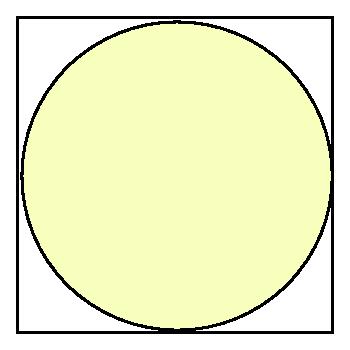
\includegraphics[width=120pt]{test.eps}
\end{center}
\caption{小さな図の例}
\end{figure}
\end{verbatim}

\begin{figure}[ht]
\begin{center}
  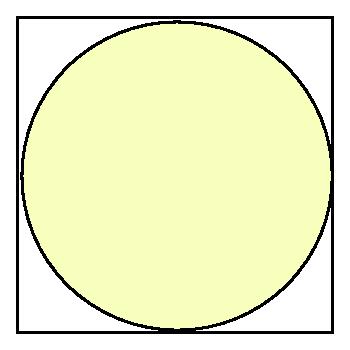
\includegraphics[width=120pt]{test.eps}
\end{center}
\caption{小さな図の例}
\end{figure}
\subsubsection*{大きな図の場合}
段をまたぐような大きな図を使用したい場合は,「小さな図の場合」で用いた
figure環境の代わりに,figure*環境を利
用します。その上で,$\backslash$includegraphicsコマンド,$\backslash$captionコ
マンドを使用し,図と図の下部に対応するcaptionが設定されるようにしてください。

\begin{verbatim}
\begin{figure}[ht]
\begin{center}
 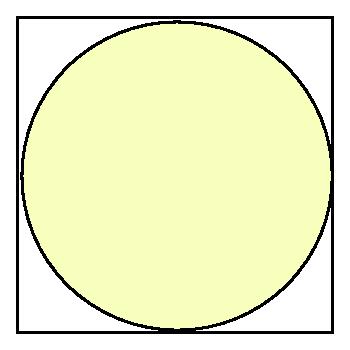
\includegraphics[width=200pt]{test.eps}
\end{center}
\caption{大きな図の例}
\end{figure}
\end{verbatim}

\begin{figure*}[ht]
\begin{center}
  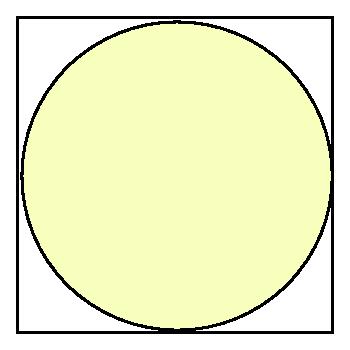
\includegraphics[width=200pt]{test.eps}
\end{center}
\caption{大きな図の例}
\end{figure*}


\subsubsection*{(2)表について}
\subsubsection*{小さな表の場合}
下記のように,table環境とtabular環境,captionコマンドを使用し,表の
下部に対応するcaptionを設定してください。

\begin{verbatim}
\begin{table}[ht!]
\begin{center}
\begin{tabular}{cc} \hline
日本語 &英語 \\ \hline
教授 & professor \\
大学院生 & graduate student \\
学部生 & undergraduate student \\ \hline
\end{tabular}
 \caption{小さな表の例}
\end{center}
\end{table}
\end{verbatim}

\begin{table}[ht!]
\begin{center}
\begin{tabular}{cc} \hline
日本語 &英語 \\ \hline
教授 & professor \\
大学院生 & graduate student \\
学部生 & undergraduate student \\ \hline
\end{tabular}
 \caption{小さな表の例}
\end{center}
\end{table}

\subsubsection*{大きな表の場合}
段をまたぐような大きな表を使用したい場合は,「小さな表の場合」で用いた
table環境の代わりに,table*環境を利
用します。その上で,tabular環境,$\backslash$captionコ
マンドを使用し,表と表の下部に対応するcaptionが設定されるようにしてください。

\begin{verbatim}
\begin{table*}[ht!]
\begin{center}
\begin{tabular}{cc} \hline
日本語 &英語 \\ \hline
教授 & professor \\
大学院生 & graduate student \\
学部生 & undergraduate student \\ \hline
\end{tabular}
 \caption{大きな表の例}
\end{center}
\end{table*}
\end{verbatim}

\begin{table*}[ht!]
\begin{center}
\begin{tabular}{cc} \hline
日本語 &英語 \\ \hline
教授 & professor \\
大学院生 & graduate student \\
学部生 & undergraduate student \\ \hline
\end{tabular}
 \caption{大きな表の例}
\end{center}
\end{table*}


\subsubsection{引用}
本文中に他の文献からの引用を含める場合には,引用符`` ''を
用いて記述してください。
1文(ないし数文)からなるような比較的短い文章を引用する場合,quote環境を用いることも可能です。
引用文が長く,独立した段落として表示する必要がある場合には,quotation環境を用いてください。
いずれの引用方法でも,末尾に
\verb|\|footnoteコマンドで,出典を記載してください。出典の記述方法に
ついては,\ref{123950_27Oct08}の「注・文献」を参考にしてください。
なお,引用した文書に番号を振る場合,閉引用符の後ろに付してください
(例えば,``~である''X。)。
出典の記述方法については,4.10の「注・文献」を参考にしてください。

\noindent{}\textbf{例1(引用符使用)}\\
澤田昭夫はよい論文について``よい論文は統一unity,連関coherence,
展開developmentにおいて優れた論文あるいは明確性clarityにおいて優れた論
文''\footnote{澤田昭夫 『論文のレトリック』 講談社, 1983, 330p, p. 19.}であると述べている。

\noindent{}\textbf{例2(quotation環境使用)}\\
澤田は論文執筆の際に次のようなことが重要だと述べている。
\begin{quotation}
論文書きでもっとも大切なのは,問を疑問文の形で切り出すことで,それがレ
 トリックで言う発見・構想です。もっとも大切だというのは,それができれば
 つまり全体を貫く主な問が何であるかを確定することができれば,論文の首尾
 一貫性,統一性を保証する基本的条件が整ったことになるからです。

そのつぎに大切なのは,論文の構成,材料の配置です。その際,肝に銘じなけれ
 ばならないのは,構成・配置の大原則は起承転結ではなく,序・本・結(序と
 本論と結び)だということです\footnote{\textit{Ibid.} p. 74}。
\end{quotation}


\subsection{注・文献} \label{123950_27Oct08}
本テンプレートファイルでは,注および文献については\verb|\|footnoteコ
マンドを
使用し,全て文末に記載します。ページごとの注(脚注)及び独立した節としての参考文献リスト(\texttt{bibitem},\texttt{bibtex}を使った記述)は用いません。
注・文献における文献の記載方法は次の例に従ってください\footnote{特に、ページ番号には En dash ( -- ; \LaTeX 上ではハイフン2個 \texttt{ --} で出力できる) を必ず用いるようにしましょう。}。
(なお,記載方
法の中で,\{\}で囲まれた項目の記述は任意です。例えば,図書の場合は``版
表示'',``出版地'',``総ページ数''が任意の記述項目です。)

\subsubsection{図書の場合}
\noindent{}和:著編者名 『書名』 \{版表示,\} \{出版地,\} 出版社, 出版年, \{総
\bigskip
ページ数,\} 当該部分のページ.\\
洋:author. \textit{title}. \{edition,\} place of publication,
publisher, year, \{total page,\} page.
\begin{quote}
 近藤二郎 『社会科学のための数学入門』 東京経済新報社, 1973,
 p. 37--40.

 Barzun, Jacques and Graff, H. F. \textit{The Modern Researcher.}
 Rev. ed., \\New York, Harcourt, 1970, p. 165.
\end{quote}


\subsubsection{翻訳書の場合}
\noindent{}和:著編者名 『書名』[原書名(イタリックで記載) \{版表示,\}
\{出版地, \} 出版社, 出版年,] 翻訳者名, 出版社, 出版年, \{総
\bigskip
ページ数,\} 当該部分のページ.\\
洋:author. \textit{title of translation}. [\textit{original
title}. \{edition,\} place of publication, publisher, year,] tr. by
translator, place of publication, publisher, year, \{total page,\} page.

\begin{quote}
Varles, Jana ed. 『情報の要求と探索』 [\textit{Information Seeking:
 Basing Services on User's Behaviors.} North Calolina,
 McFarland \& Company, 1987] 池谷のぞみ, 市古健次, 白石英理子, 田村俊作訳,
 勁草書房, 1993, p. 10.

Schneider, Georg. \textit{Theory and History of Bibliography.}
 [\textit{Handbuch der Bibliographie.} Aufl., Berlin, Knopt, 1978,]
 tr. by R. R. Shaw, New York, Columbia University Press, 1934, p. 14--15.
\end{quote}

\subsubsection{編集書の一部(図書形態の論文集の一論文を含む)の場合}
\noindent{}和:当該部分の執筆者名 ``当該部分の題名'' $<$編者名 『書名』 \{版表示,\} \{出版地,\} 出版社, 出版年$>$ \{総
\bigskip
ページ数,\} 当該部分のページ.\\
洋:author. ``\textit{title},'' in editor. \textit{book title}, \{edition,\} place of publication,
publisher, year, \{total page,\} page.

\begin{quote}
宮坂広作 ``余暇と社会教育'' $<$碓井正久編著 『社会教育』 第一法規,
 1970$>$ p. 201--203.

Groom, Geofrey. ``\textit{Bibliography of older material},'' in Garvin,
 L. H. ed. \textit{Printed Reference Material.} 2nd ed., London, Library
 Association, 1984, p. 456--501.
\end{quote}


\subsubsection{逐次刊行物掲載記事(雑誌論文を含む)の場合}
\noindent{}和:執筆者名 ``論題名'' 『掲載逐次刊行物名』 vol. XX,
\{no. XX,\} 発行年\{月\}, 当該部分のページ.\\
洋:author. ``title,'' \textit{name of periodical}, vol. XX,
\{no. xx,\} year \{month\}, page.


\begin{quote}
小野寺夏生 ``Bibliostatistics'': 情報現象の統計学的説明'' 『情報管理』
 vol. 21, no. 10, 1979, p. 782--802.

小野寺夏生, 中井浩 ``単純なモデルからのZipfの法則の導入'' 『情報科学技術
 研究集会論文集』 vol. 33, no. 3, 1977, p. 129--138.

Brookes, Bertram C. ``Theory of the Bradford Laws,'' \textit{Journal of
 Documentation,} vol. 33, no. 3, 1977, p. 180--209.

Nelson, Micheal J. and Tague, Jean M. ``Sprit Size-Rank Models for the
 Distribution of Index Terms,'' \textit{Journal of the American Society
 for Information Science,} vol. 36, no. 5, 1985, p. 283--296.
\end{quote}

\subsubsection{Web上のリソースについて}
Web上のリソースについては,書誌情報の最後に入手先URLとアクセスした日付を記入します。
書式は``入手先URL: http://www.p.u-tokyo.ac.jp/(アクセス日: 2008-10-27 )''または
(``available from http://www.p.u-tokyo.ac.jp/ (accessed date: 2008-10-27)'')を記入します。
それ以外の項目は図書並びに逐次刊行物掲載記事の規定に準じ,入手先の情報から明らかである項目を記述します。

\begin{quote}
 情報メディア学会. 『『情報メディア研究』への各種原稿の投稿について』 入手
 先URL: http://www.jsims.jp/toko.html (アクセス日: 2008-10-27)
\end{quote}

\subsubsection{書誌事項の記載における省略語の使用について}

同一文献を二度以上引用する場合は,和文文献,欧文文献どちらの場合でも,
\textit{op. cit.}(前掲文献の意)\textit{Ibid.}(上掲文献の意)を用います。
こちらはイタリック体(斜字体)の代わりに下線を用いても良いこととします。
な\textit{op. cit.}を用いる場合,name,\textit{op. cit.}, (year,) p. Xのように記載します。
\textit{Ibid.}を用いる場合については,本文末注3の使用例を参照してください。


\subsection{文章末の要約情報}
論文等の最後には,改ページを行った後,本文を記述した言語以外のタイトル,
著者名,所属,要約,キーワード情報を記載します。本文を日本語で作成
した場合は,英文の情報を,本文を英文で記述した場合は,日本語の情報を記載
することになります。

\LaTeX{}の場合には,テンプレートファイルの最後に英文要約作成エリ
アが用意されています。テンプレートファイル上では,以下の箇所が該当します。

\small{}
\begin{verbatim}
%--------------------------------------
%英文要約作成用エリア(\eauthors,
%\eaffiliation,\etitle,
%\eabstract,\keywordの欄を書き換えて使う)
%--------------------------------------
\newpage
\twocolumn[
\begin{center}
\etitle{Manual of Writing a Manuscript for
Articles, Research Notes, and
 Materials in \textit{Studies in Lifelong
Learning Infrastructure Management}}
\begin{eauthors}
\name{1}{Yahoi HONGO} \name{2}{Tarou TOUDAI}
\end{eauthors}
\begin{eaffiliation}
\eaff{1}{Graduate School of Education,
the University of Tokyo}
 \eaff{2}{Society for Lifelong Learning
Infrastructure Management}
\end{eaffiliation}
 \begin{eabstract}
The paper describes style and layout of
manuscripts in \textit{the Studies in
Lifelong Learning Infrastructure
Management}. You can use directly this
  file when you make your manuscript.
 \end{eabstract}
\begin{keyword}
Keyword: Studies in Lifelong Learning
Infrastructure Management, Script Manual, Layout
\end{keyword}
\end{center}
]
\end{verbatim}
\normalsize

\subsubsection{作成エリア上の必須環境,必須コマンド}
まず,作成エリア直後のおよび末尾の以下のコマンドは,文章整形のために必要
な記述ですので,削除しないでください。
\begin{verbatim}
\newpage
\twocolumn[
\begin{center}
\end{verbatim}
......
\begin{verbatim}
\end{center}
]
\end{verbatim}


\subsubsection{英文タイトル}
論題に対応する英文タイトルを記入します。\verb|\|etitleコマンドの引数
に対応するタイトルを記入してください。
タイトルにはsentence caseを用いてください。文頭の単語と文中の固有名詞の先頭のみを大文字とする書き方です。

\begin{verbatim}
\etitle{Manual of writing a manuscript
for articles, research notes, and
materials in \textit{Studies in Lifelong
Learning Infrastructure Management}}
\end{verbatim}

\subsubsection{英文著者名}
英語で著者名を名姓の順で記入します(名は頭文字のみ大文字,姓は全て大文字)。\verb|\|eauthors環境の
中に,\verb|\|nameコマンドが含まれています。コマンドの引数は第1引数
に何番目の著者かを記入し,第2引数には著者名を記入します。ま
た,\verb|\|nameコマンドを書いた数だけ,著者名と対応する記号が付与される
ようになっています。


テン
プレートファイル上では,著者が2名存在する場合のサンプルを記入していま
す。著者が1名の場合には,\verb|\|nameコマンドの\{2\}\{\}以降を削除し
\verb|\|name\{1\}\{\}の部分だけを使用してください。著者が3名以上いる
場合には,\verb|\|nameコマンドを著者の人数分増やして,順序に応じて
\verb|\|nameコマンドの最初の引数を変更して使用してください。例え
ば,3人の場合には以下のようになります。
\begin{verbatim}
\begin{eauthors}
\name{1}{Yayoi HONGO}
\name{2}{Tarou TOUDAI}
\name{3}{Komaba KASHIWA}
\end{eauthors}
\end{verbatim}
本テンプレートファイルでは著者名を5つまで記入することができます。著者
名欄が6つ以上必要な場合は,スタイルファイルの改変が必要ですので,事
前にご連絡下さい。


\subsubsection{英文所属}
著者に対応する英文所属を記入します。\verb|\|eaffiliation環境の中に,
\verb|\|eaffコマンドが含まれています。コマンドの引数は第1引数に所属
の記述順(\verb|\|nameコマンドの第1引数と対応させてください)を記入
し,第2引数には所属の英文名を記入します。


テン
プレートファイル上では,著者が2名存在する場合のサンプルを記入しています。も
し,著者が1名の場合には,\verb|\|eaffコマンドの\{2\}\{\}以降を削除し
\verb|\|name\{1\}\{\}の部分だけを使用してください。第3著者以降がいる
場合には,\verb|\|eaffコマンドを著者の人数分増やして,順序に応じて
\verb|\|eaffコマンドの最初の引数を変更して使用してください。例え
ば,3人の場合には以下のようになります。

\begin{verbatim}
\begin{eaffiliation}
\eaff{1}{Graduate School of Education,
the University of Tokyo}
\eaff{2}{Society for Lifelong Learning Infrastructure
 Management}
\eaff{3}{Another Organization}
\end{eaffiliation}
\end{verbatim}
本テンプレートファイルでは所属を5つ
まで記入することができます。所属欄が6つ以上必要な場合は,スタイルファ
イルの改変が必要ですので,事前にご連絡下さい。

なお,「東京大学大学院教育学研究科」の英文所属は``Graduate School of
Education, the University of
Tokyo''で統一するようお願いいたします。

\subsubsection{英文要約}
論文の内容に対する要約を英文で記入します。下記のサンプルのように,
eabstract環境の中に要約を\textbf{100語から150語で}記入してください。


\begin{verbatim}
 \begin{eabstract}
The paper describes style and layout of
manuscripts in the Studies in \textit{
Lifelong Learning Infrastructure
Management}.
You can use directly this
file when you make your manuscript.
 \end{eabstract}

\end{verbatim}


\subsubsection{英文キーワード}
論文の内容に対するキーワードを記入します。下記のように,
keyword環境の中に適切なキーワードを英語で\textbf{3つ程度}記入して
ください。文中の冠詞と前置詞と接続詞を除いて,各語の先頭は大文字とします。

\begin{verbatim}
\begin{keyword}
Keywords: Studies in Lifelong Learning
Infrastructure Management,
Script Manual, Layout
\end{keyword}
\end{verbatim}


%--------------------------------------
%注エリアの作成用コマンド(消さないこと!)
%--------------------------------------
\begingroup \parindent 0ex \parskip 0.5ex \def\ennotesize{\normalsize}
\theendnotes \endgroup
%--------------------------------------
%英文要約作成用エリア(\eauthors,\eaffiliation,\etitle,
%\abstract, \keywordの欄を書き換えて使う)
%--------------------------------------
\newpage
\twocolumn[

\begin{center}
\etitle{Manual of writing a manuscript for articles, research notes, and
 materials in \textit{Studies in Lifelong Learning Infrastructure Management}}
\begin{eauthors}
\name{1}{Yahoi HONGO} \name{2}{Tarou TOUDAI}
\end{eauthors}
\begin{eaffiliation}
\eaff{1}{Graduate School of Education, the University of Tokyo}
 \eaff{2}{Society for Lifelong Learning Infrastructure Management}
\end{eaffiliation}
 \begin{eabstract}
The paper describes style and layout of manuscripts in \textit{the Studies in
  Lifelong Learning Infrastructure Management}. You can use
  directly this
  file when you make your manuscript.
 \end{eabstract}
\begin{keyword}
Keywords: Studies in Lifelong Learning Infrastructure Management, Script Manual, Layout
\end{keyword}
\end{center}
]


\end{document}
